\documentclass[12pt]{article}
\usepackage{graphicx}


\title{TOF Command-line Tool: User Manual}
\author{Aly Aly}
\begin{document}
\maketitle
\section{Purpose of Tool}
The purpose of this tool is to process direct event data files produced during IMAP-Lo calibrations. This tool is intended for use by any test operator or designated analysis team to create TOF histograms is 1D and 2D. For those reasons the only required input is a filepath to a DE$\_$RAW file produced by IMAP-Lo GSEOS in .csv format.

\section{Quick Start}

\subsection{Installation}
\label{subsec:qckstrt}
To install this tool download the tool folder where you want it. Make sure you have a the following packages installed:
none
, for now. Then you are ready to use the tool.

\subsection{Fastest way to plot...}

\subsubsection{Everything} 
\label{subsubsec:everything}
Type the following in you favorite powershell/terminal from inside that directory. 

\begin{verbatim}
python /path/to/tool/command_line_tool.py -f /path/to/file/XXX_RAW_DE_######_.csv

\end{verbatim}
Replace /path/to/file/ and /path/to/tool/ with the paths on your machine. This command alone will produce plots in 2D of the data in the .csv file provided. The data will not be cleaned in anyway, i.e. all singles and doubles are plotted as well. The files will be saved in the same directory as the input file. Unless we specify the output file path, including the name, with the -o option, all plots are saved in the same directory as the input file. As an example if the .csv file is in a directory called test$\_$data, the plots and a new .csv will be saved there as well. To find out more about -o see Section \ref{subsubsec:qs_out}.


\subsubsection{Triples and Golden triples (-v and -ch)} 

To make the same plots for triples then type the following code.

\begin{verbatim}
python command_line_tool.py -f XXX_RAW_DE_######_.csv -v 1 1 1 1

\end{verbatim}

for golden triples:

\begin{verbatim}
python command_line_tool.py -f XXX_RAW_DE_######_.csv -v 1 1 1 1 -ch

\end{verbatim}

, where the checksum filter is a conditional.
\begin{verbatim}
if abloute_value_of_checksum > 1 , then discard_event

\end{verbatim}

To change the value of the checksum filter to 0.5 instead of 1, use the following code.
\begin{verbatim}
python command_line_tool.py -f XXX_RAW_DE_######_.csv -v 1 1 1 1 -ch 0.5

\end{verbatim}

\subsection{Output location and naming (-o and -st).}
\label{subsubsec:qs_out}
 To put all output in a dirctory other than the input file the use the -o flag 
 \begin{verbatim}
 python command_line_tool.py -f \path\to\csv\csv_filename.csv -o .\path\to\out\filenames_prefix
 \end{verbatim}
 
 This code will create all the output from Section \ref{subsubsec:everything} for file /path/to/csv/csv$\_$filename.csv in  directory /path/to/csv/ and all files will have "filenames$\_$prefix" as the first part of the name. default is to use the input filename without the .csv. Some times the plot names are too long to use as figure titles so we can use the -st option to give the figures a title since default is "filenames$\_$prefix". 
 \begin{verbatim}
 python command_line_tool.py -f \path\to\csv\csv_filename.csv -o .\path\to\out\filenames_prefix -st "Figure_title_here"
 \end{verbatim}
 
 

\section{.csv file format}
This tool ingests contents of a file produces by IMAP-Lo GSEOS. The files ingested have the string "DE$\_$RAW" in the file name. These files consist of rows that include the DE block with 500 counts maximum per block or row (see figure .

\begin{figure}[h]
\caption{Example of a .csv file with DE$\_$RAW in file name }
\centering
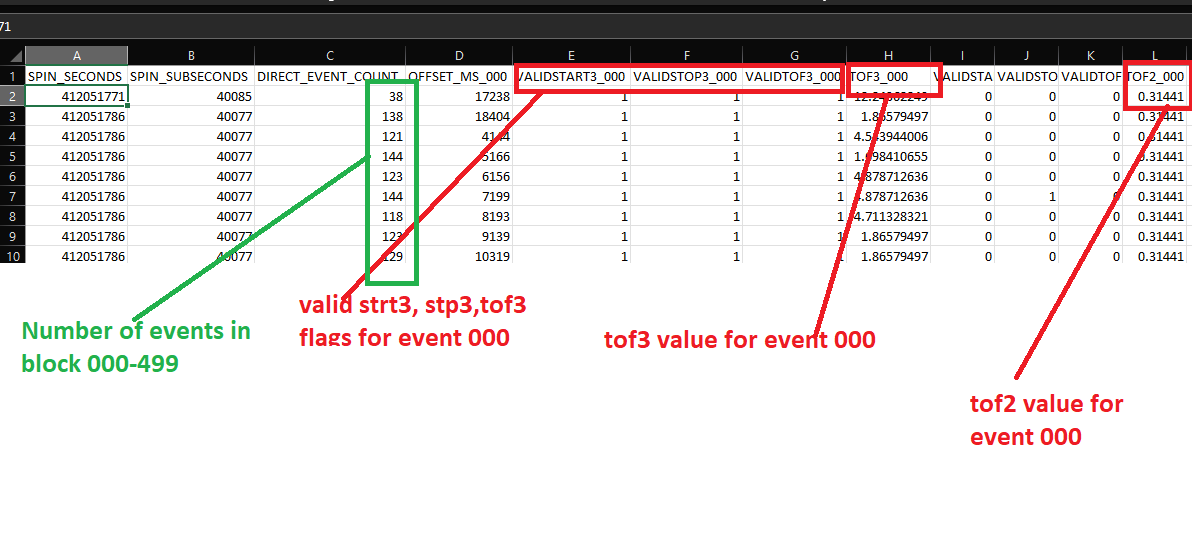
\includegraphics[width=1\textwidth]{csv1}
\end{figure}


\end{document}